\chapter{Dataset Analysis}

\justifying

Let us recall that the ultimate goal is to build a binary classifier capable of determining whether a piece of source code was written by a human or generated by a Large Language Model (LLM). For binary classifiers, \textbf{accuracy} is typically the default evaluation metric, unless one classification outcome, such as true positives or false positives, is considered more critical than the other. Given that this classifier can be used in scenarios where a programmer could be 'accused' of not having authored the code themselves, it is essential that such claims be made with a high degree of confidence. While it is certainly desirable to allow end users to configure the decision threshold, the default setting should prioritize a \textbf{low FPR} (false positive rate) to prevent unjust accusations.

\section{Dataset Evaluation Criteria}



All datasets made publicly available by the scientific 
community will be carefully analysed and compared. 
The goal is to identify the most suitable dataset—either 
directly or through integration, for the evaluation of code 
detection methods under consistent conditions. Each dataset 
will be assessed based on the following criteria:

\begin{enumerate}
    \item \textbf{Total number of code samples available:} 
    a larger number of samples generally improves statistical 
    robustness during evaluation and model training.
    
    \item \textbf{LLMs used to generate synthetic code:} 
    datasets that include code generated by multiple LLMs are better 
    suited for evaluating a method’s generalization capability.
    \begin{enumerate}
        \item \textbf{Number of LLMs:} 
        to avoid a method from focusing too much on 
        stylistic features of a specific LLM, it is essential 
        to have codes generated by different LLMs.
        \item \textbf{Actual degree of use in contemporary times:}
        while it is desirable for detection methods to have 
        long-term viability, it is undeniable that a detector 
        effective on current LLMs (such as GPT-4 \cite{openai2023gpt4}) is more useful 
        than one targeting outdated models (such as GPT-3 \cite{brown2020language}).
        \item \textbf{Actual types diversity among LLMs:}
        it is also necessary to analyse the diversity of the models 
        themselves. For instance, it is more informative to include 
        in the same dataset code produced by both an open-source LLM 
        like CodeLlama\cite{roziere2023code} 
        and a commercial one like GPT-3 \cite{brown2020language}, rather than, for 
        example, code from GPT-3 \cite{brown2020language} 
        and Codex \cite{chen2021codex} (which is itself based on GPT-3).
    \end{enumerate}
    
    \item \textbf{Code diversity:} 
    ensuring diversity in the code is essential to understand 
    how generalizable a method is to the overall code domain, 
    or whether it is specialized in the stylistic patterns of 
    specific LLMs \textit{(a particularly relevant issue for methods relying 
    on stylistic features of the code)}.
        \begin{enumerate}
        \item \textbf{Different programming languages:}
        while Python is currently the most relevant language 
        in the field of artificial code generation (indeed, many 
        datasets primarily consist of Python code 
        such as MBPP \cite{austin2021program}), 
        it is valuable 
        to evaluate detection methods across as many programming 
        languages as possible. At the very least, it is worth 
        assessing different detection methods on different languages, 
        possibly recommending specific approaches depending 
        on the language being analysed.
        \item \textbf{Different types of code:}
        although language differences are important, 
        they are not sufficient. Python, for example, 
        can be used both as an object-oriented and a procedural 
        language. Understanding the type of code being analysed 
        can aid both in training and in evaluating a detector.
        \item \textbf{Code size:}
        code length is a key parameter, as the ease of identifying 
        the origin of the code may vary depending on its size. 
        It is worth noting that in certain contexts, such as homework 
        assignments, short code snippets are extremely common.
        \item \textbf{Code context:}
        it is useful to include examples 
        of human-written code from both competitive settings 
        (such as Leetcode dataset \cite{xia2025leetcodedataset}) 
        and open-source project environments 
        (such as CodeSearchNet \cite{husain2019codesearchnet}), 
        in order to evaluate detectors across different real-world contexts.
    \end{enumerate}

    \item \textbf{Validity information:} 
    this includes whether the dataset provides information on the 
    validity of human-written code, the exact prompts used to generate 
    LLM code, or whether code quality and correctness have been validated.
    \begin{enumerate}
        \item \textbf{Generation prompts:}
        it may be useful to evaluate the different 
        prompts used to generate the code, as it is 
        well known that varying the prompt can lead to 
        significantly different outputs from an LLM.
        \item \textbf{Source of human-written code:}
        many datasets are based on collections of human-written 
        code that are later used to generate LLM outputs. Knowing 
        the source of this human code ensures the reliability 
        and correctness of the dataset.
        \item \textbf{Code quality:}
        performing tests such as verifying whether 
        both human and LLM-generated code actually 
        works is essential. \textit{There is little value in 
        analysing whether non-functional code was 
        produced by an LLM or not.}
        \item \textbf{Paper reliability:} 
        This point is important for preprinted papers, 
        for which reliance on the scientific community is 
        not possible.
    \end{enumerate}

\end{enumerate}


Although all these are evaluation parameters, it is natural that some 
are more relevant than others: knowing the source of the human-written 
code remains more important than simply including a few additional LLMs 
in the code generation process.

\clearpage
\section{Datasets Proposed in the Scientific Literature}
The works whose main contribution is the 
creation of a dataset are mostly preprints, 
and thus require careful consideration. 
The papers primarily dedicated to dataset 
generation include: CoDet-M4 \cite{orel2025codet}, 
AIGCodeSet \cite{demirok2024aigcodeset}, 
and CodeMirage \cite{guo2025codemirage}.

\subsection*{CoDet-M4}
The main contribution of this work is the construction 
of a dataset derived from existing human-written code datasets, 
by generating synthetic code using six different LLMs. 
The authors then train several models on this dataset 
to evaluate their performance, 
demonstrating that their dataset can significantly improve 
the effectiveness of various code detection models.
The authors employ the following models as code generators:

\begin{itemize}
    \item \textbf{GPT-4o}: A proprietary model developed by OpenAI, selected to represent the state-of-the-art among large-scale, closed-source LLMs.
    
    \item \textbf{CodeLlama (7B)}: An open-source model by Meta, specifically trained for code-related tasks. It is one of the most popular code-oriented language models.
    
    \item \textbf{Llama3.1 (8B)}: A more recent version of Meta’s Llama family. Although it is a general-purpose model, it exhibits strong performance in code generation.
    
    \item \textbf{CodeQwen 1.5 (7B)}: An open-source model from Alibaba Cloud, also specialized in code, and part of the Qwen series.
    
    \item \textbf{Nxcode-orpo (7B)}: A fine-tuned variant of CodeQwen. The authors include it to evaluate the robustness of detectors against different fine-tuning strategies applied to the same base model (in this case, ORPO – Monolithic Preference Optimization).
\end{itemize}


\subsubsection*{Strengths}
\begin{itemize}
    \item The introduction of one of the most extensive and diverse datasets proposed for the task of LLM-generated code detection.
    \item Dataset cleaning is carefully performed, including the use of \textit{Codeforces} as one of the tools to assess the correctness of human-written code {(\scriptsize\textit{Section 3.3: Quality Assurance})}.
    \item The authors also construct an ``out-of-domain'' dataset, specifically designed to contain code with characteristics intentionally different from the main dataset {(\scriptsize\textit{Section 4.4:Out-of-Domain Experiment})}.
    \item The dataset includes code in three different programming languages, unlike other works that focus solely on Python {(\scriptsize\textit{Section 3.1: Data Collection})}.
\end{itemize}

\subsubsection*{Weaknesses}
\begin{itemize}
    \item Suspiciously high in-domain classification metrics, with F-scores exceeding 98\% {(\scriptsize\textit{Table 2})}.
    \item The prompts used to generate synthetic code vary depending on the source, potentially introducing an unintentional correlation between code types and the generation prompts {(\scriptsize\textit{Appendix F})}.
    \item Most of the LLMs used for code generation are lightweight models, with GPT-4o being the only large-scale LLM involved {(\scriptsize\textit{Section 3.2: Code Generation})}.
\end{itemize}


Once the dataset is downloaded from the \href{https://huggingface.co/datasets/DaniilOr/CoDET-M4}{official portal}, 
several important features are found to be missing:
\begin{enumerate}
    \item The declared train/validation/test split described in the paper is not included; only the test set is provided. This makes \textbf{reproducing their results more difficult}.
    \item Some significant \textbf{code-level features are missing}, such as whether the code sample is class-based or function-based.
    \item The authors state in the paper that they plan to keep updating the dataset, which may explain small discrepancies in the number of code samples compared to what is reported. For example, there are fewer GitHub samples than those claimed in the original publication.
\end{enumerate}


\begin{figure}[H]
    \centering
    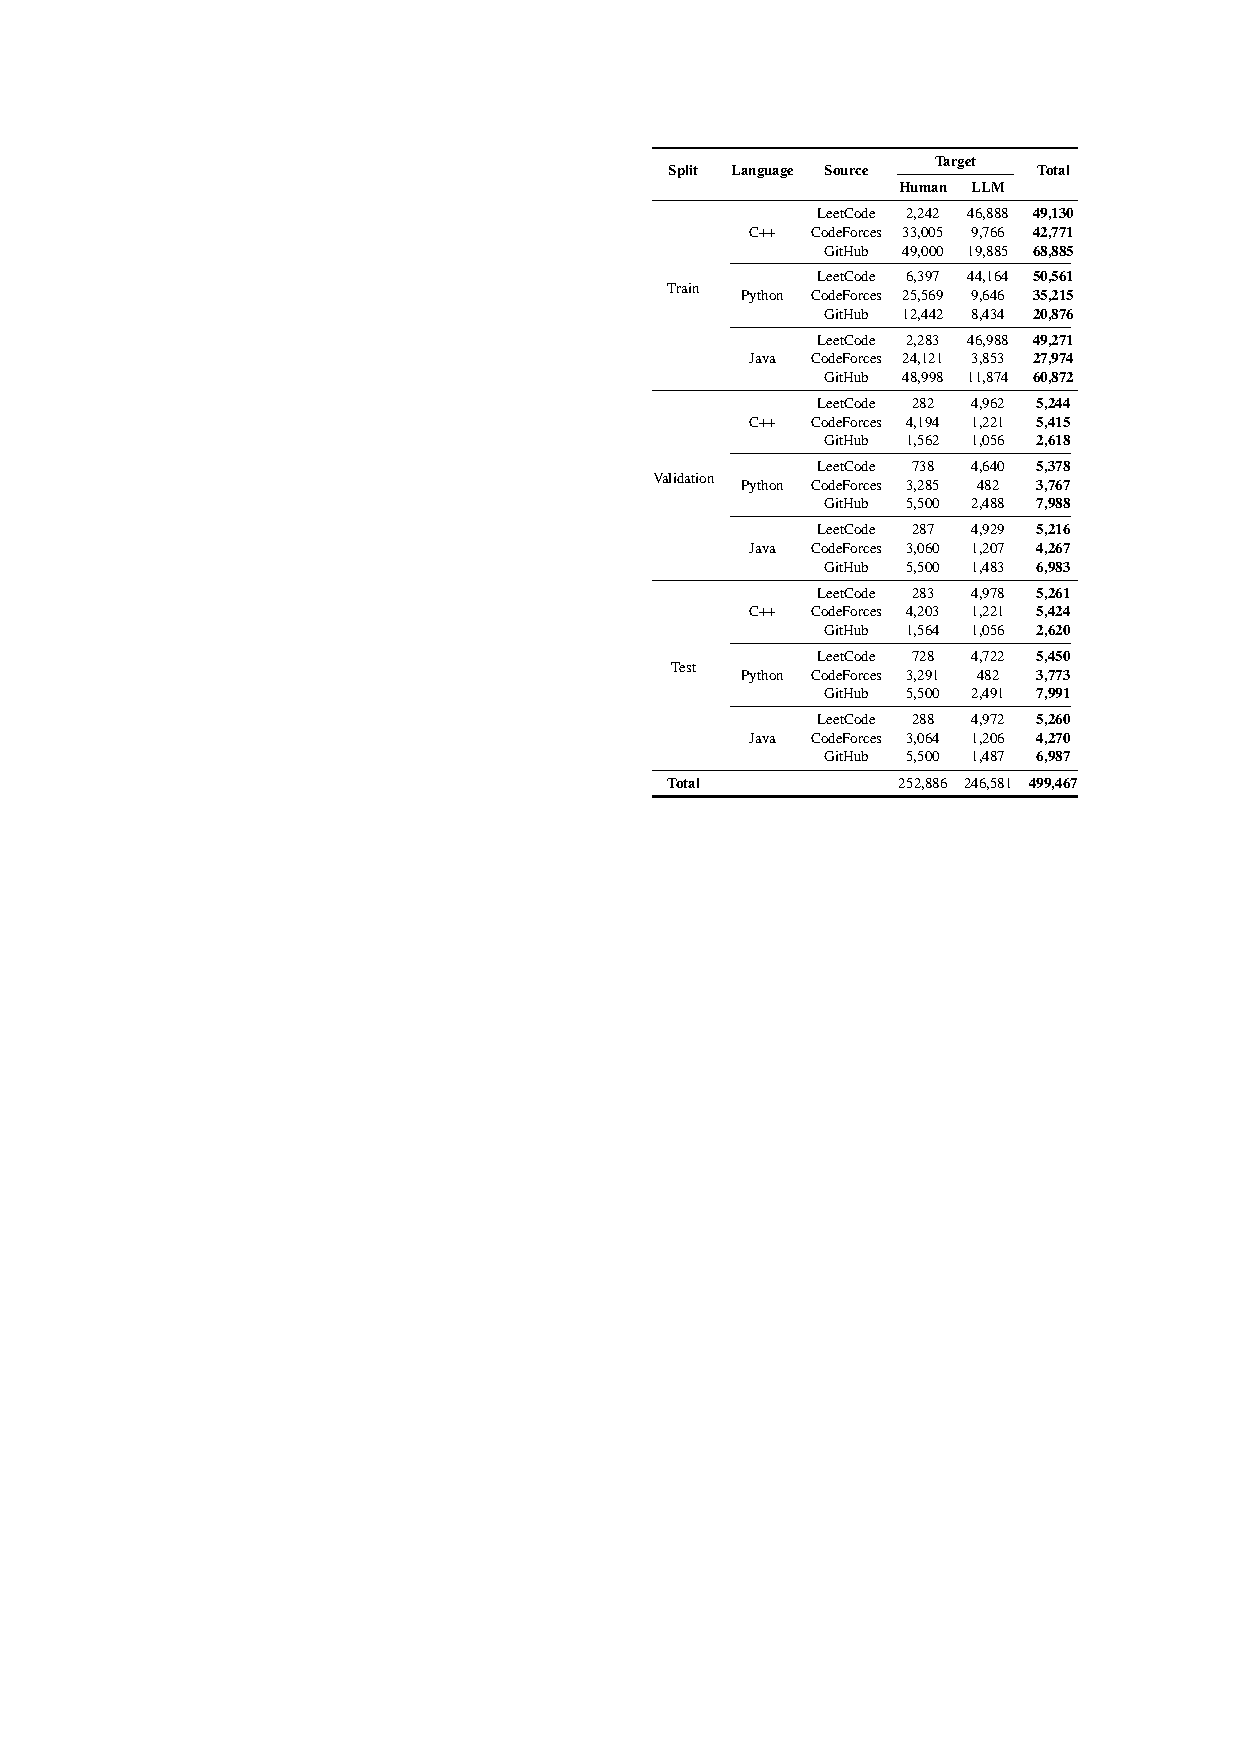
\includegraphics[width=0.5\textwidth]{img/CoDet-M4/tab1.pdf} % Inserisci il nome corretto del file immagine
    \caption{Table 1 \cite{orel2025codet}: Number of code snippets in train/val/test sets}
    \label{fig:table1_CoDet-M4}
\end{figure}

\clearpage
\section{Final Dataset}